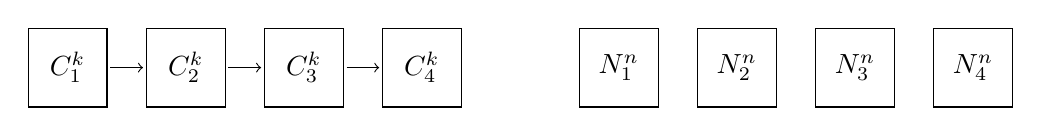
\begin{tikzpicture}
    \node[style=draw, minimum width=1cm, minimum height=1cm] (c1) at (0, 0) {$C^k_1$};
    \node[style=draw, minimum width=1cm, minimum height=1cm] (c2) at (1.5, 0) {$C^k_2$};
    \node[style=draw, minimum width=1cm, minimum height=1cm] (c3) at (3, 0) {$C^k_3$};
    \node[style=draw, minimum width=1cm, minimum height=1cm] (c4) at (4.5, 0) {$C^k_4$};

    \node[style=draw, minimum width=1cm, minimum height=1cm] (n1) at (7, 0) {$N^n_1$};
    \node[style=draw, minimum width=1cm, minimum height=1cm] (n2) at (8.5, 0) {$N^n_2$};
    \node[style=draw, minimum width=1cm, minimum height=1cm] (n3) at (10, 0) {$N^n_3$};
    \node[style=draw, minimum width=1cm, minimum height=1cm] (n4) at (11.5, 0) {$N^n_4$};

    \draw[->, shorten >=1pt, shorten <=1pt] (c1) -- (c2);
    \draw[->, shorten >=1pt, shorten <=1pt] (c2) -- (c3);
    \draw[->, shorten >=1pt, shorten <=1pt] (c3) -- (c4);
\end{tikzpicture}